%% Creator: Inkscape inkscape 0.48.0, www.inkscape.org
%% PDF/EPS/PS + LaTeX output extension by Johan Engelen, 2010
%% Accompanies image file 'param_vs_dir.eps' (pdf, eps, ps)
%%
%% To include the image in your LaTeX document, write
%%   \input{<filename>.pdf_tex}
%%  instead of
%%   \includegraphics{<filename>.pdf}
%% To scale the image, write
%%   \def\svgwidth{<desired width>}
%%   \input{<filename>.pdf_tex}
%%  instead of
%%   \includegraphics[width=<desired width>]{<filename>.pdf}
%%
%% Images with a different path to the parent latex file can
%% be accessed with the `import' package (which may need to be
%% installed) using
%%   \usepackage{import}
%% in the preamble, and then including the image with
%%   \import{<path to file>}{<filename>.pdf_tex}
%% Alternatively, one can specify
%%   \graphicspath{{<path to file>/}}
%% 
%% For more information, please see info/svg-inkscape on CTAN:
%%   http://tug.ctan.org/tex-archive/info/svg-inkscape

\begingroup
  \makeatletter
  \providecommand\color[2][]{%
    \errmessage{(Inkscape) Color is used for the text in Inkscape, but the package 'color.sty' is not loaded}
    \renewcommand\color[2][]{}%
  }
  \providecommand\transparent[1]{%
    \errmessage{(Inkscape) Transparency is used (non-zero) for the text in Inkscape, but the package 'transparent.sty' is not loaded}
    \renewcommand\transparent[1]{}%
  }
  \providecommand\rotatebox[2]{#2}
  \ifx\svgwidth\undefined
    \setlength{\unitlength}{230.01171875pt}
  \else
    \setlength{\unitlength}{\svgwidth}
  \fi
  \global\let\svgwidth\undefined
  \makeatother
  \begin{picture}(1,1.4490634)%
    \put(0,0){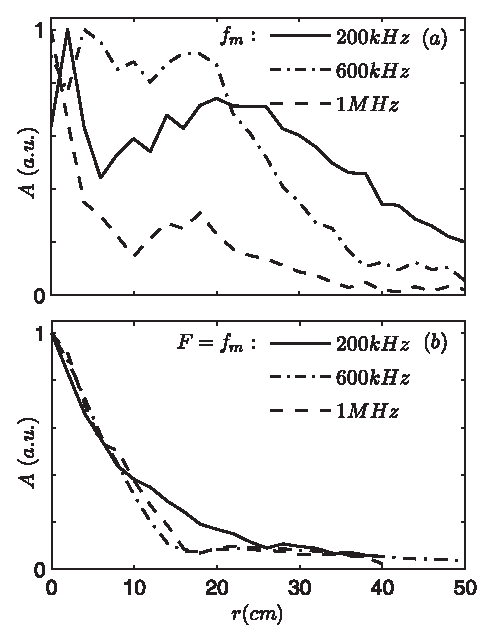
\includegraphics[width=\unitlength]{pics/param_vs_dir.eps}}%
    \put(0,-0.05){\color[rgb]{0,0,0}\makebox(0,0)[lb]{\smash{$0$}}}%
    \put(0.18,-0.05){\color[rgb]{0,0,0}\makebox(0,0)[lb]{\smash{$10$}}}%
    \put(0.372,-0.05){\color[rgb]{0,0,0}\makebox(0,0)[lb]{\smash{$20$}}}%
    \put(0.578,-0.05){\color[rgb]{0,0,0}\makebox(0,0)[lb]{\smash{$30$}}}%
    \put(0.769,-0.05){\color[rgb]{0,0,0}\makebox(0,0)[lb]{\smash{$40$}}}%
    \put(0.968,-0.05){\color[rgb]{0,0,0}\makebox(0,0)[lb]{\smash{$50$}}}%
    \put(0.44,-0.1){\color[rgb]{0,0,0}\makebox(0,0)[lb]{\smash{$r$\,(см)}}}%
    \put(0.7,0.37){\color[rgb]{0,0,0}\makebox(0,0)[lb]{\smash{$1$\,МГц}}}%
    \put(0.7,0.45){\color[rgb]{0,0,0}\makebox(0,0)[lb]{\smash{$600$\,кГц}}}%
    \put(0.7,0.53){\color[rgb]{0,0,0}\makebox(0,0)[lb]{\smash{$200$\,кГц}}}%
    \put(0.9,0.54){\color[rgb]{0,0,0}\makebox(0,0)[lb]{\smash{$(б)$}}}%
    \put(0.32,0.532){\color[rgb]{0,0,0}\makebox(0,0)[lb]{\smash{$F=f_m:$}}}%
    \put(-0.04,-0.01){\color[rgb]{0,0,0}\makebox(0,0)[lb]{\smash{$0$}}}%
    \put(-0.04,0.58){\color[rgb]{0,0,0}\makebox(0,0)[lb]{\smash{$1$}}}%
    \put(0.7,1.26){\color[rgb]{0,0,0}\makebox(0,0)[lb]{\smash{$200$\,кГц}}}%
    \put(0.7,1.186){\color[rgb]{0,0,0}\makebox(0,0)[lb]{\smash{$600$\,кГц}}}%
    \put(0.7,1.104){\color[rgb]{0,0,0}\makebox(0,0)[lb]{\smash{$1$\,МГц}}}%

    \put(0.9,1.264){\color[rgb]{0,0,0}\makebox(0,0)[lb]{\smash{$(а)$}}}%
    \put(-0.04,0.65){\color[rgb]{0,0,0}\makebox(0,0)[lb]{\smash{$0$}}}%
    \put(-0.04,1.27){\color[rgb]{0,0,0}\makebox(0,0)[lb]{\smash{$1$}}}%
    \put(-0.06,0.9){\color[rgb]{0,0,0}\rotatebox{90}{\makebox(0,0)[lb]{\smash{$A$\,(у.е.)}}}}%
    \put(-0.06,0.23){\color[rgb]{0,0,0}\rotatebox{90}{\makebox(0,0)[lb]{\smash{$A$\,(у.е.)}}}}%
    \put(0.442,1.268){\color[rgb]{0,0,0}\makebox(0,0)[lb]{\smash{$f_m$:}}}%
  \end{picture}%
\endgroup
